\section{The Model}

\frame
{
	\begin{center}
		\LARGE The Model: Evolution of Mimicry
	\end{center}
}

\frame
{
	\frametitle{The Model}
	\framesubtitle{Evolution of Mimicry}
	
	\begin{itemize}
		\item \textbf{Objective:} Build an \textit{agent based} Artificial Life model for simulating the evolution of mimicry.	
		\item Two species of agents:
			\begin{enumerate}
				\item Prey
					\begin{itemize}
						\item Model
						\item Mimic
					\end{itemize}
				\item Predator
			\end{enumerate}
		\item Prey pattern representation: Cellular Automata.
		\item Predator pattern recognition: Hopfield Network.
		\item Environment: Visual representation, 3D, toroidal.
	\end{itemize}	
}

\subsection{Past Work}

\frame
{
	\frametitle{The Model}
	\framesubtitle{Past Work}

	\begin{itemize}
		\item Turner(1996) and Huheey(1988):
			\begin{itemize}
				\item \textbf{Focus:} Selective pressure on prey, by learning ability of predator.
				\item Predators use simple Monte Carlo learning or mathematical approach.
			\end{itemize}
		\item Sherratt(2002):
			\begin{itemize}
				\item Co-evolving predator and prey population.
				\item Predators are deterministic, cannot learn from experience.
				\item Predators attack policy is fixed, either attack or avoid.
			\end{itemize}
	\end{itemize}
}

%-------------------------------
%More slides on Franks and Noble
%-------------------------------

\frame
{
	\frametitle{Past Work}
	\framesubtitle{Franks and Noble}

	\begin{itemize}
		\item First Model(2002):
			\begin{itemize}
				\item \textbf{Focus:} 
				\item Predators use simple Monte Carlo learning or mathematical approach.
			\end{itemize}
		\item Second Model(2004):
			\begin{itemize}
				\item Co-evolving predator and prey population.
				\item Predators are deterministic, cannot learn from experience.
				\item Predators attack policy is fixed, either attack or avoid.
			\end{itemize}
	\end{itemize}
}

%-------------------------------
%More slides on Franks and Noble
%-------------------------------

\subsection{FormAL}

\frame
{
	\frametitle{FormAL Framework}
	
	\begin{itemize}
		\item Ideas from Peter Grogono's Formal Artificial Life (FormAL) project.
		\item \textbf{Goal:}		
			\begin{itemize}
				\item To study the emergence of complexity.
				\item No variable unless genetically controlled or influenced. \textit{Principal not followed for Hopfield Network.}
			\end{itemize}
		\item \textbf{Agents:}
			\begin{itemize}
				\item Simulated organism.
				\item Able to reproduce itself using genetic information.
				\item Capable of modifying structures of genome between generations.
				\item Able to interact with other agents.
				\item Survive and reproduce in a challenging environment.
			\end{itemize}
	\end{itemize}
	
}

\frame
{
	\frametitle{FormAL Framework}
	\framesubtitle{Environment}
	
	Environment is 3D, where agents get complete freedom of movement defined from genetic representation.
	\begin{itemize}
		\item \textbf{Space:}
			\begin{itemize}
				\item 3D Lattice of discreet points.
				\item \((x,y,z) \in \Sigma^3\), where \(\Sigma\) be the set \(\{0, 1, ..., S-1\}\).
				\item \(S\) is a universal constant, small positive number. Value is 20, \(World Size\) parameter. 
			\end{itemize}
		\item \textbf{Time:}
			\begin{itemize}
				\item Integer value, increases in discreet steps. 
				\item Each agent updates itself in each time step.
			\end{itemize}
		\item \textbf{Cell:}
			\begin{itemize}
				\item Entire environment is divided into multiple cells.
				\item A 3D cubical section of the hyperspace.
				\item \(ISize\) parameter kept at 6. Total \(ISize^3 = 216\) cells.
			\end{itemize}
	\end{itemize}
}

\frame
{
	\frametitle{FormAL Framework}
	\framesubtitle{Environment Parameters}
	
	\begin{table}[H]
	\centering
	\begin{spacing}{1.5}
	\begin{scriptsize}
%	\begin{tabular}{| p{2.2cm} | >{\centering} p{3cm} | p{7.5cm} |}
	\begin{tabular}{| p{1.5cm} | >{\centering} p{2cm} | p{4cm} |}
		\hline
			\textbf{Parameter} & \textbf{Value} & \textbf{Description} \\ \hline
			ISize & 6 & Number of cell in single dimension of the 3-D toroidal cube\\ \hline
			World Size & 20 & Size of a single dimension of the 3-D toroidal cube\\ \hline
			Cell Size & \( World Size / ISize \) & Size of each cell\\ \hline
			Total Number of Cells & \( ISize^3  = 216\) & Total number of cells in the environment\\ 
		\hline
	\end{tabular}
	\end{scriptsize}
	\end{spacing}
	\caption{Parameters to control the environment.}
	\label{tab:environment-control-parameters}
	\end{table}
}

\frame
{
	\frametitle{FormAL Framework}
	\framesubtitle{Environment - Visual representation - Front}

	\begin{figure}[H]
		\centering
		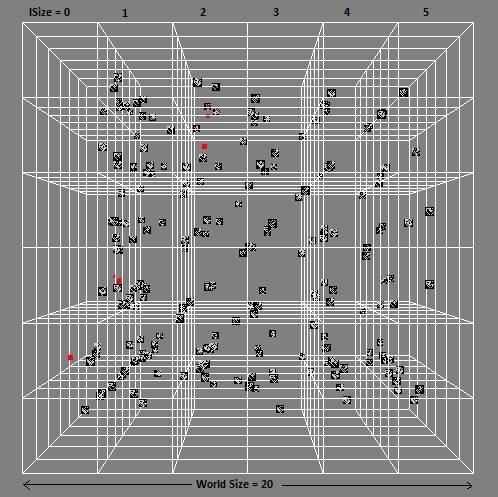
\includegraphics[scale=0.40]{../tex/images/cells-front}
		\caption{Three dimensional representation of the environment divided in cells. Presence of different species of agents inside.}
	\label{tab:3-d-environment-images-1}
	\end{figure}	
}

\frame
{
	\frametitle{FormAL Framework}
	\framesubtitle{Environment - Visual representation - Top}

	\begin{figure}[H]
		\centering
		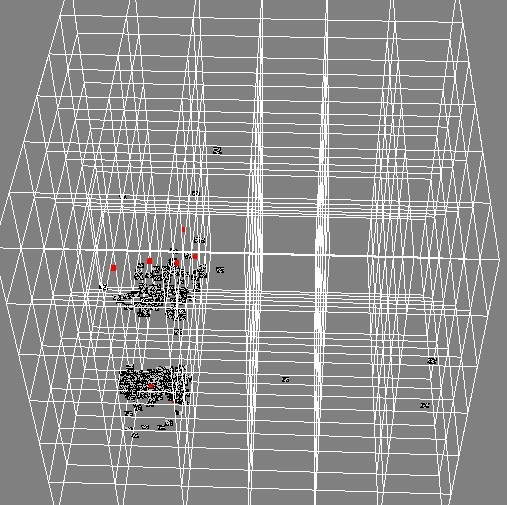
\includegraphics[scale=0.40]{../tex/images/cells-top}
		\caption{Three dimensional representation of the environment divided in cells. Presence of different species of agents inside.}
	\label{tab:3-d-environment-images-2}
	\end{figure}	
}

\frame
{
	\frametitle{FormAL Framework}
	\framesubtitle{Environment - Visual representation - Side}

	\begin{figure}[H]
		\centering
		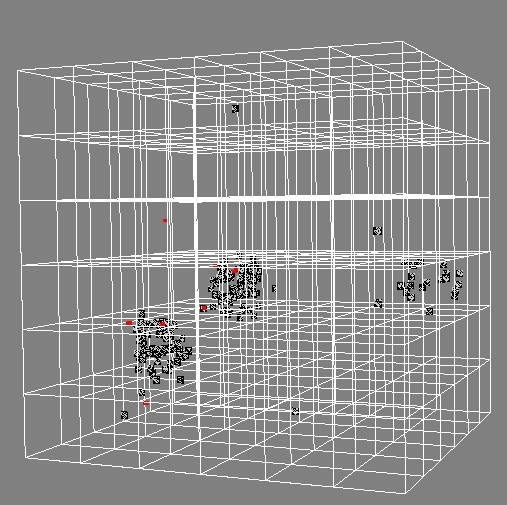
\includegraphics[scale=0.40]{../tex/images/cells-side}
		\caption{Three dimensional representation of the environment divided in cells. Presence of different species of agents inside.}
	\label{tab:3-d-environment-images-3}
	\end{figure}	
}

\frame
{
	\frametitle{FormAL Framework}
	\framesubtitle{Agent Mobility}
	
	\begin{itemize}
		\item Position is calculated in each step in time.
		\item \(position\), \(force\), \(acceleration\) and \(velocity\) are all vector components.
		\item \(force\) is calculated from the mobility genes.
		\item Newton's law of motion is used to calculate \(acceleration\) when \(force\) is not zero.
		\item \(acceleration\) is integrated to obtain velocity and new position.
	\end{itemize}

}

\frame
{
	\frametitle{FormAL Framework}
	\framesubtitle{Mobility Parameters}

	\begin{table}
	\centering
	\begin{scriptsize}
	\begin{spacing}{1.5}
	\begin{tabular}{| p{1.7cm} | >{\centering} p{0.6cm} | p{5cm} |}
		\hline
			\textbf{Parameter} & \textbf{Value} & \textbf{Description} \\ \hline
			Force Factor & 40 & A unit vector is multiplied by this amount before being added to the force vector.\\ \hline
			Differential Time Step (DT) & 0.01 & The time step used for first-order integration of the motion equations.\\ \hline
			Friction & 5 & The friction constant used for motion calculations.\\ \hline
			Work Factor & 1 & \( Work done = WF * force * distance \), where \(WF\) is this constant.\\
		\hline
	\end{tabular}
	\end{spacing}
	\end{scriptsize}
	\caption{Parameters to control mobility of agents.}
	\label{tab:mobility-control-parameters}
	\end{table}
	
}

\subsection{Prey}

\frame
{
	\frametitle{The Prey: Mimics and Models}
	\framesubtitle{Pattern Representation}

	\begin{figure}[H]
		\centering
		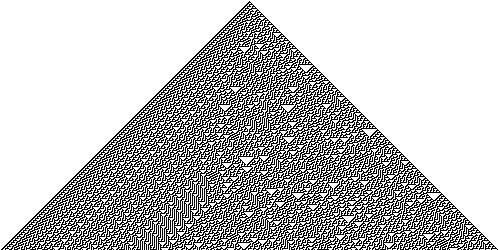
\includegraphics[scale=3]{../tex/images/CA_rule30s}
		\caption{Cellular Automata Rule 30.
		Image source: \href{http://en.wikipedia.org/wiki/Cellular_automata}{Wikipedia}}
		\label{fig:cellular-automata-rule-30}
	\end{figure}
	
	\begin{table}
		\centering
		\begin{scriptsize}
		\begin{tabular}{| p{2cm} | c | c | c | c | c | c | c | c |}
		  \hline
		  Current Pattern & 111 & 110 & 101 & 100 & 011 & 010 & 001 & 000 \\ \hline
		  New state of center cell & 0 & 0 & 0 & 1 & 1 & 1 & 1 & 0 \\
		  \hline
		\end{tabular}
		\end{scriptsize}		
		\caption{Cellular Automata rule}
		\label{tab:cellular-automata-rule}
	\end{table}
}

\frame
{
	\frametitle{The Prey: Mimics and Models}
	\framesubtitle{Species Diversity}

	\begin{itemize}
		\item Agent's pattern genome is 8 bit binary value.
		\item Decimal range 0 to 255.
		\item 256 unique CA pattern associated.
		\item The linear representation of this pattern is stored in Hopfield Network.
		\item Hamming distance between a pattern's linear representation is used to consider similarity.
		\item Group of prey with a specific pattern is considered in a single species.
		\item Inter species reproduction is restricted to control diversity of patterns.
		\item Using ``Pattern Mutation Rate" we control diversity of new species.
	\end{itemize}
}

\frame
{
	\frametitle{The Prey: Mimics and Models}
	\framesubtitle{Genome}
	
	\begin{itemize}
		\item 17 bit prey Genome
	\end{itemize}
	
	\begin{table}[H]
	\centering
	\begin{scriptsize}
	\begin{spacing}{1.5}
	\begin{tabular}{|c|c|c|c|}
		\hline
			\textbf{Pattern(8)} & \textbf{Palatability(2)} & \textbf{Mobility(6)} & \textbf{Reproduction(1)} \\ \hline
			10101101					 	& 							01		 		 & 			110001					&					1						 		 \\ \hline
	\end{tabular}
	\end{spacing}
	\end{scriptsize}
	\caption{Distribution and purpose of each gene of the 17 bit prey genome.}
	\label{tab:prey-genome}
	\end{table}
}

\frame
{
	\frametitle{The Prey: Mimics and Models}
	\framesubtitle{Punctuated Equilibrium}
	
	\begin{itemize}
		\item Punctuated Equilibrium:
			\begin{itemize}
				\item inclined to cladogenesis instead of gradualism.
				\item Turner emphasizes on punctuated equilibrium to explain evolution of mimicry.
				\item CA pattern evolution is in a single mutation in the pattern genome.
				\item Change of pattern is not a gradual process but rather an arbitrary discontinuous one.
			\end{itemize}
	\end{itemize}
}

\frame
{
	\frametitle{The Prey: Mimics and Models}
	\framesubtitle{Mobility}
	
	\begin{itemize}
		\item Six bit of the mobility gene is used to calculate the magnitude of force for mobility.
		\item Direction is decided based on 
			\begin{itemize}
				\item Towards collection of maximum prey species in a cell.
				\item Away from concentration of predators.
				\item Move towards the selected cell with the magnitude of force calculated.
			\end{itemize}
	\end{itemize}
}

\frame
{
	\frametitle{The Prey: Mimics and Models}
	\framesubtitle{Reproduction}
	
	\begin{itemize}
		\item Reproduction begins at ``Reproductive Age"
		\item Reproduction capability is decided on 17th bit gene.
		\item Mate selection is random, but within same cell.
		\item Mate needs to be
			\begin{itemize}
				\item similar species
				\item genetically capable to reproduce
				\item reached maturity 
			\end{itemize}
		\item Reproduction process:
			\begin{itemize}
				\item Single point crossover.
				\item Two point mutation is applied based different rates.
					\begin{itemize}
						\item \textit{Pattern Mutation Rate}
						\item \textit{Genome Mutation Rate}
					\end{itemize}
			\end{itemize}
	\end{itemize}
}

\frame
{
	\frametitle{The Prey: Mimics and Models}
	\framesubtitle{Configuration Parameters}
	
	\begin{table}[H]
	\centering
	\begin{scriptsize}
	\begin{tabular}{| p{1.5cm} | >{\centering} p{1cm} | p{4cm} |}
		\hline
			\textbf{Parameter} & \textbf{Value} & \textbf{Description} \\ \hline
			Prey Size & 2 to 5 & Size of the prey species in the 3D FormAL  environment.\\ \hline
			Reproduction age limit & 100 & Minimum number of iterations or time steps a prey species need to be present in the simulation to get reproduction capability\\ \hline
			Reproduction interval & 1000 & Number of iterations a prey need to wait before reproducing again.\\ \hline
			Pattern Mutation Rate & 0.05 & Rate of Mutation of the pattern genome.\\ \hline
			Genome Mutation Rate & 0.5 & Rate of mutation of the rest of the genome excluding the pattern gene.\\ \hline
			Demise Age & 2000 & Age at which the prey species will be removed from the environment.\\
		\hline
	\end{tabular}
	\end{scriptsize}
	\caption{Parameters to control prey population and visibility.}
	\label{tab:prey-control-parameters}
	\end{table}
}

\subsection{Predator}

\frame
{
	\frametitle{The Predator}
	
	\begin{itemize}
		\item Agent in the FormAL environment.
		\item Provide selection pressure for the evolution of mimicry.
		\item Each agent equipped with Hopfield Network Memory.
		\item Mobility and reproduction capability controlled genetically.
		\item Unable to represent pattern recognition capability with genome.
		\item New predators are born with zero memory, as memory is not inherited.
	\end{itemize}
}

\frame
{
	\frametitle{The Predator}
	\framesubtitle{Learning}

	\begin{itemize}
		\item Predator's interaction objective with prey is consumption.
		\item Consumption is based on palatability.
		\item If unable to consume prey is thrown back into environment.
		\item At this event prey pattern is stored into predators memory with the associated palatability.
		\item New pattern learned with Hebbian Learning.
	\end{itemize}
}

\frame
{
	\frametitle{The Predator}
	\framesubtitle{Hebbian Learning}

	\begin{itemize}
		\item Initially all weights are set to zero.
		\item Use Hebbian rule to calculate outer product of input-output vector pair, for each pair.
		\item The Outer vector matrix of all the patterns are summed to come up with the final weight matrix.
	\end{itemize}
	
Each component of the weight matrix \(\textbf{W} = \{w_{ij}\}\) is given by:
\begin{equation}
w_{ij} = \sum_{p=1}^{P} s_i(p) t_j(p), i \neq j
%\label{eq:}
\end{equation}
\[
w_{ij} = 0, i = j
\]
where P is the number of patterns. Vectors \textbf{S} and \textbf{T} are respectively, the input and the desired output of the network.

}

\frame
{
	\frametitle{The Predator}
	\framesubtitle{Design of Memory}
	
	\begin{itemize}
		\item Input to Memory:
			\begin{itemize}
				\item Each prey has an evolving CA represented by a binary Genome.
				\item This 2D pattern is serialized to a 1D binary array.
				\item Binary representation is converted to bipolar representation.
			\end{itemize}
		\item Pattern Recognition with Hopfield Network:
			\begin{itemize}
				\item Learning: Apply Hebbian learning to calculate weights.
				\item Initialization: Input to the network is initialized with value of the input vector.
				\item Iterate Until Convergence: Each neuron is updated asynchronously with the input of its previous state until convergence.
				\item Output: Finally a pattern is set as output when the network reaches convergence.
			\end{itemize}
	\end{itemize}
}

\frame
{
	\frametitle{The Predator}
	\framesubtitle{Attack Algorithm}
	
	\begin{itemize}
		\item When agent reaches `Minimum Attack Age' it starts hunting.
		\item Select a random prey within vicinity (same cell).
		\item Attack process involves recognition of prey pattern.
		\item Two parameters to limit pattern memorization and recognition process as both are computationally expensive.
			\begin{itemize}
				\item Hopfield Minimum Memory Size (value 2 to 6)
				\item Hopfield Maximum Memory Size (value 10)
			\end{itemize}
		\item New predator attacks without caution. 
		\item Attacks everyone and in the process store pattern and palatability.
		\item When memory reaches `Hopfield Minimum Memory Size': intelligent selection.
	\end{itemize}
}

\frame
{
	\frametitle{The Predator}
	\framesubtitle{Genome}

	\begin{table}
	\centering
	\begin{scriptsize}
	\begin{spacing}{1.5}
	\begin{tabular}{|c|c|}
		\hline
			\textbf{Mobility(4)} & \textbf{Reproduction(1)} \\ \hline
					 1101					   &					1						 		\\ \hline
	\end{tabular}
	\end{spacing}
	\end{scriptsize}
	\caption{Distribution and purpose of each gene of the 5 bit predator genome.}
	\label{tab:predator-genome}
	\end{table}
}

\frame
{
	\frametitle{The Predator}
	\framesubtitle{Mobility}
	
	\begin{itemize}
		\item First 4 bits of the genome calculated to evaluate the magnitude of force of movement.
		\item Direction is decided based on the number of prey species present in a neighboring cell.
		\item Move towards the cell with least number of predator and most number of prey.
		\item This is such that predators are distributed all over the environment.
		\item Increases agent's predatory behavior.
	\end{itemize}
}

\frame
{
	\frametitle{The Predator}
	\framesubtitle{Reproduction process}
	
	\begin{itemize}
		\item Agent reaches reproduction age.
		\item Agent exceeds reproduction age interval, which is difference in time between two reproduction activity.
		\item Agent is capable of reproduction depending on 5th gene.
		\item Select another predator from same cell which satisfy above conditions.
		\item Perform crossover and mutation to create another predator.
		\item Predator is initialized with zero memory.
	\end{itemize}
}

\frame
{
	\frametitle{The Predator}
	\framesubtitle{Configuration Parameters}
	
	\begin{table}
	\centering
	\begin{tiny}
	\begin{tabular}{| p{1.3cm} | >{\centering} p{0.8cm} | p{5cm} |}
		\hline
			\textbf{Parameter} & \textbf{Value} & \textbf{Description} \\ \hline
			Minimum Memory Size & 2 to 6 & Minimum number of patterns stored in memory before predators start making intelligent decisions.\\ \hline
			Maximum Memory Size & 10 & Maximum number of patterns to be stored in memory. Limited to reduce processing time. \\ \hline 
			Hopfield Maximum Iterations & 20 & Maximum number of iterations for Hopfield Network to recognize a pattern. Usually the network reaches a steady state before that. But this restriction is to avoid infinite loop in case the network never reaches a steady state. \\ \hline
			Attack Age & 500 & minimum age a predator needs to reach to be able to attack prey species.  \\ \hline
			Attack Interval & 100 & Interval of time which needs to pass before a predators attacks its next prey. \\ \hline
			Genome Mutation rate & 0.3 & Mutation rate for the 5 bit genome of the predators representing their mobility and pattern recognition capability. \\ \hline
			Reproduction Age Limit & 500 & Minimum age a predator needs to reach before engaging in reproduction.\\ \hline
			Reproduction Interval & 1000 to 3000 & Interval of time a predator needs to pass between two reproduction process.\\ \hline
			Demise Age & 2000 to 7000 & Age at which a predator is considered as dead.\\
		\hline
	\end{tabular}
	\end{tiny}
	\caption{Parameters to control predator population and pattern recognition capability.}
	\label{tab:predator-control-parameters}
	\end{table}
}